\documentclass[12pt]{article}

\usepackage[margin=1in]{geometry}
\usepackage{xcolor}
\usepackage{graphicx}
\usepackage{url}
\usepackage{hyperref}
%\usepackage{ulem}

\newcommand\TODO[1]{\textcolor{red}{#1}}
\newcommand\todo[1]{\textcolor{red}{#1}}

\begin{document}
\title{Fine-grained Access Control for NFC Applications}
\author{Max Feldman \and Stephanie Rogers \and Richard Xia}
\maketitle

\begin{abstract}
Near Field Communication (NFC) is a form of contactless communication that allows devices to transfer data over radio; it is similar to RFID, but with a much smaller range of use.
NFC has existed for some time, but its implementation in Android phones, along with an API for developers, has only recently gained popularity.
%Upon scanning an NFC tag, Android will automatically run the application that has been associated with the type of data on that tag, often without user interaction or approval.
Alarmingly, several applications implement features such as SMS messaging or calling given phone numbers, or accessing arbitrary URLs, which are provided by an NFC tag without even prompting the user.
%The Android NFC API offers application developers a new, more powerful means to access NFC capabilities in mobile devices, but this introduces an increased attack space and additional potential for vulnerability.
%Android provides access to an NFC Data Exchange Format (NDEF) API, but does not offer any of the various security measures that have been proposed by the NFC standards group (the NFC Forum).

We examine the growing space of NFC applications offered for Android, and provide a categorization of the functionality and general security practices of these applications.
We address the issue of authorization of NFC tags by providing fine-grained access control based on data type and author.
We discuss known issues and vulnerabilities with NDEF security, and how our proposal mitigates some of these concerns.
We also keep in mind the importance of usability, especially in applications that minimize user interruption---as is the case with NFC applications.
%Finally, we present the description of a user study that can effectively evaluate the tradeoffs between secure access control and usability.
\end{abstract}

%\tableofcontents

\section{Introduction}
NFC-enabled devices have existed for several years, but with NFC deployment in Android phones developers have more power to write NFC applications than was previously available.
The growing prevalence of NFC devices, and the developer-friendly nature of Android in particular, lead to a rapidly expanding space of NFC Android applications\footnote{\url{http://www.frost.com/sublib/display-report.do?id=9843-00-13-00-00}}.
This expansion of applications and functionality may be a sign of an expansion of the attack surface as well.

In this paper, we frame the state of NFC vulnerabilities and proposed solutions, and evaluate the practicality of these solutions for Android devices.
More and more, we see feature-rich applications which perform actions based upon NFC data which is read from an NFC tag or tag emulator.
This allows for useful functionality and fast, responsive applications, but it also raises concerns regarding untrusted NFC data.
For example, some Android applications offer the ability to automatically call a phone number if they receive an NFC input specifying a phone number.
If this application were to be fed a malicious NFC input specifying a paid phone number, then the user's phone could make a call which charged the user's cellular account, all without the user's knowledge.
There are NFC protocols to provide digital signatures, but Android currently does not implement these, nor do they sufficiently protect against several types of attacks \cite{roland2011, nfcsignaturertd}.
Additionally, there is no standard means of determining authorization after NFC data is authenticated.

We identify other NFC-related threats, among them both threats which are in the scope of this paper, and threats which we do not discuss.
Android allows users to write NFC tags (and transmit NFC data) in addition to performing read operations.
This allows for richer applications, but also raises concerns regarding users sharing sensitive data over NFC (which is by default unencrypted).
Although there are protocols and proposals for secure data transfer over NFC, Android does not support these either \cite{nfcsignaturertd, nfcsec01}.
Both reading and writing of NFC data in Android is insecure, and developers currently must implement their own security solutions if they wish to offer security for these operations.

We propose a solution to the issue of authorization, in the form of access control lists for NFC data.
We describe a system which attempts to maximize usability and security of reading in NFC data, by allowing users to manage which tag authors they trust in a given context.
We describe the operations present in this system, and how the OS both handles marshalling NFC data after verifying access policies, as well as the utilities provided to the user for access control management.
NFC security in Android applications has not previously been thoroughly addressed; we seek to rectify this and provide a feasible solution to some potential NFC attack vectors.
%There are other means of providing similar NFC security, and we address the merits of select alternatives to our proposal.

In order to evaluate the efficacy of our proposal, we implement basic functionality of our recommended system.
This requires emulating NFC digital signature standards which Android does not yet support, but we show that a simple API can provide powerful additional security.

In our future work, we discuss further additions to our system which would be helpful, including additional encryption to protect user privacy when transmitting NFC data.
This is not a new idea, but Android currently lacks support for secure transmission, outside of the developer linking cryptographic methods with NFC methods on their own.
Were Android to provide integration of NFC and cryptographic protocols, it would reduce developer work as well as the risk of developers improperly employing cryptography.
We also pose goals for a future user study which could illuminate user response to our system, and how well our access control integrates with real applications and use cases.

\section{Background}
Near Field Communication (NFC) is an emerging technology for wireless communication that allows NFC-enabled devices to transfer small amounts of data at a close proximity, usually no more than a few centimeters \cite{nfcip-1, nfcip-2}.
At the most basic level, NFC specifies a set of protocols for this wireless communication based off of the radio-frequency identification (RFID) standards.

NFC-enabled devices can use the protocol in two modes: active and passive.
In passive mode, there is a device actively generating a radio frequency (RF) field that initiates contact to the passive NFC tag.
An NFC tag is a passive device that stores data for NFC transmission.
There are several types of NFC tags, but in general they are a means of persistent storage for NFC data.
Depending on the type of tag, the data can be overwritten or modified, or require authentication from a reader before transmitting its data \cite{koninggans2008}.
In this case, the device can read or write information stored on NFC tags and cards without the passive targets needing any power source.
Active devices are also able to emulate passive NFC tags by transmitting NFC data to a receiver which is acting as an active device.
For the purpose of discussion within this paper, we use ``tag'' to refer to either a physical tag, or a device which is emulating a tag, as their functionality is the same within the context of our exploration.
Additionally, NFC phones have the ability to communicate with other NFC-enabled mobile phones to transfer data peer-to-peer in active mode.
In this case both devices are generating their own RF fields.

\subsection{Android NFC}
The Android system sends and receives NFC data in the form of NFC Data Exchange Format (NDEF) messages.
These messages, which are stored in the NFC tag, act as a container for one or more NDEF records which are further broken up into a header and a payload.
NDEF records also contain a header which contains two fields for describing the payload type: ``Type Name Format (TNF)'' and ``Type''.
TNF is a 3-bit field which specifies the format of the type; a TNF value of 1 indicates a well-known type (defined by the NFC Forum) and a TNF value of 2 indicates a MIME-type, for example.
Descriptions of the other TNF values can be found in the official specification \cite{ndef}.
Type is field of arbitrary length which more precisely describes the type of the data in the NDEF record.
Type can refer to a well-known type, such as a URI, or text, or it can refer to a MIME-type or custom application type, for example.
An example breakdown of an NDEF message can be found in Figure~\ref{fig:background:ndef}

\begin{figure}[h!]
	\centering
		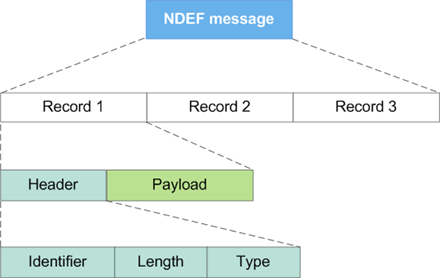
\includegraphics[width=0.5\textwidth]{NDEF_Format.png}
	\caption[Caption for LOF]%
		{NDEF Message Format. Figure adapted from \\{\scriptsize\url{http://www.developer.nokia.com/Community/Wiki/Understanding_NFC_Data_Exchange_Format_(NDEF)_messages}}}
  \label{fig:background:ndef}

\end{figure}

Specifically, the Android system offers the ability to read and write NFC tags for passive mode, and beam NDEF messages from one device to another with Android Beam.\footnote{\url{http://developer.android.com/guide/topics/connectivity/nfc/nfc.html}} for active mode. 

\subsection{Android Intents}
\label{sec:background:intents}
The core components of an Android application are activated through messages called intents.\footnote{\url{http://developer.android.com/guide/components/intents-filters.html}}
Intents are used for inter-application and intra-application communication by sending messages with relevant information about operations to be performed to various applications.  

When NFC is enabled and the screen is unlocked, Android devices will always be searching for input from an NFC tag or device. 
When the device discovers an NFC tag, the Android OS creates an intent that is dispatched to an application that has registered for a tag of that type.
This information is processed by Android's special tag dispatch system to determine which activity to launch.
In the case that more than one application can handle the type of data contained in the tag, the phone will open a prompt for the user to choose among the several applications; however, if there is only one application, the phone will automatically launch this application and process the tag.
NFC input can force Android phones (with certain settings) to parse images, videos, contacts, and office documents, call or text arbitrary phone numbers, establish Bluetooth connections, and open web pages via the browser, all without user interaction.  

\subsection{Android Permission System}
\label{sec:androidperm}
Android applications run in a sandbox that allows areas of the system to be isolated and thus limit access to the security-related parts of the Android API.
However, access to these resources can be granted to an application if the developer requests the appropriate permissions in the application's manifest.
Android developers are expected to limit the permissions requested to only those that are absolutely necessary for the function of their applications.
Access to the NFC hardware is a permission that application developers must request, and many applications which request NFC permission also require other permissions such as Internet access and making phone calls.
As of writing this report, there were 253 free NFC-enabled Android applications available for download.
We examined the applications to determine which permissions they used.
Of these applications, 78\% had the Internet permission, 18\% had the permission to place a phone call, and 10\% had the permission to send an SMS message.

\section{Threat Model}
While NFC is still an emerging technology, there are several vulnerabilities that can afflict applications.
In our work, we primarily address the threat of malicious NFC tags, but also consider threats to a user's privacy. 

\subsection{Malicious Tags}
We define a malicious NFC tag as an NFC tag that contains data that would cause a user to act on data in a way that they did not expect.
If the attacker has the ability to call to an arbitrary number, then the attacker could call a tolled number and thus result in a monetary loss on the part of the user. 
An example of an application that does this is Samsung's Tectile\footnote{\url{http://www.samsung.com/us/microsite/tectile}} application which, when scanning a tag with a phone number and directions to call this number, will do so without any further user prompts.
For example, an attacker could replace the tag on a poster advertising a local event with a new tag containing a paid phone number.
When a user swipes the tag to view the event's website, the user's phone will place a call and will be billed for the call.

\subsection{Privacy Concerns}
\label{sec:threatmodel:privacy}
Several NFC applications have the possibility of writing information to an NFC tag.
This means that users have the ability to write anything they want to their own tags.
It may be beneficial for some users to use these tag-writing applications to write sensitive or critical information to tags they keep in specific locations.
However, if encryption is not used, an attacker who can gain access to these tags will have unfettered access to their information.
For example, under certain conditions the Tectile application will write the email address of the user to the tag, unencrypted.
Tectile uses this as a means of authenticating a tag (we will not discuss the flaws of such an authentication scheme), which means that if a user enables a setting in Tectile, their email address will automatically be written to all future tags they write.
NFC is also used as a means of initiating connections on higher-bandwidth media (eg. Bluetooth), but if this connection handover is interfered with then an attacker may be able to listen in on the new connection.

\subsection{Unaddressed Threats}
There are several other threats to consider, which we mention here, but are outside the scope of our project.
In \cite{kortvedt2009}, Kortvedt, proves that it is possible to eavesdrop on NFC communication using simple equipment and methods.
Since the NFC communication protocol does not offer any security or encryption itself, it is up to the developer to implement or use encryption to secure the data within the application's code. 
Our proposal and implementation do not address the issue of eavesdropping, but we consider the mitigation of this problem in Section~\ref{sec:futurework}.

We also omit discussion of relay, replay, and denial of service attacks because our solution only solves the problem of authorization.

\section{Relevant NFC Technology and Security}
It is important to address the related technology to NFC and some of the protocols implemented and proposed that already attempt to deal with the above NFC issues. 

MiFare, FeliCa and AFAICT are all contactless smart cards that can acts as tags for NFC devices and each offer different security features.
MiFare is hardware that can restrict read and write access to only individuals with a pre-shared key.
FeliCa provides authentication and write protection as well.
AFAICT has the ability to lock the data to make it not overwritable, but does not provide authentication.
As each type of tag only offers a subset of the security measures that are possible, it is left to the developer to provide some sort of security scheme or use cryptography to provide privacy. 
These protocols allow a tag to authenticate and authorize a device, whereas our solution allows a device to authorize a tag.


\section{Related Work}
%Close range radio wave communication has existed for some time, but the application of NFC in mobile phones is a recent development and still growing in popularity.
The NFC Forum\footnote{\url{http://www.nfc-forum.org/}}, which publishes NFC standards\footnote{\url{http://www.nfc-forum.org/specs/spec_list/}} and best practices, was formed in 2004.
The relative youth of this field has resulted in many aspects remaining largely unexplored.
In this section we present relevant past work in the area of NFC security, as well as mobile phone application security in general.

\textbf{Pre-shared keys.}
One approach for authenticating tags is to share keys between tag readers and tag writers.
Kortvedt \cite{kortvedt2009} proposes a general framework for providing one-way and mutual authentication over NFC, but requires the use of pre-shared keys.
He suggests using a centralized key authority associated with mobile carriers such as Over-The-Air (OTA) programming or SMS for distributing keys.
We believe it is impractical and inappropriate for all types of applications given that tag authors may be distinct from application authors and may wish to distribute keys.
There is also no notion of trust, as a user must trust that the key being shared is legitimate.
We instead seek to provide a decentralized mechanism for trusting and granting trust to a user-defined set of NFC tag authors.

\textbf{Signatures and Certificates.}
The NFC Signature Record Type Definition (RTD), which can be used to sign NDEF records, was standardized to deal with threats caused by malicious tags including spoofing, phishing and denial of service.
A signature record can be used to sign individual records or contiguous groups of records in an NDEF message, as shown in Figure~\ref{fig:relatedwork:signature}.
\begin{figure}[h!]
\begin{minipage}{\textwidth}
	\centering
		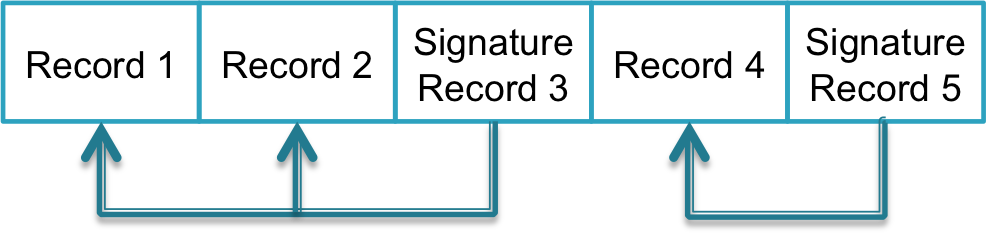
\includegraphics[width=0.5\textwidth]{signed_ndef.png}
	\caption[Caption for LOF]%
  {An NDEF message in which signature record 3 signs records 1 and 2, and signature record 5 signs record 4.}
  \label{fig:relatedwork:signature}

\end{minipage} 
\end{figure}

Using signatures on a tag results in a performance and space penalty, which are important since NFC tag readers are mobile devices and NFC tags themselves have very limited storage space \cite{kilas2009}.
The standard now focuses on being able to authenticate the source of data through a certificate authority which distributes and validates public keys \cite{rosati2011}.
However, vulnerabilities arise with these signature records when mixing signed and unsigned records in a single NDEF message \cite{roland2010,roland2011}.
We propose a way for users to authorize keys based on the data type and application, which are enough to determine a fixed behavior (e.g. calling a phone number from a tag or opening a URL stored on a tag).

\textbf{Network Vulnerabilities}
In addition to the security that various NFC technologies have provided, there has been much insight into the vulnerabilities of NFC at the network-level. 
One major foray into such analysis was presented by Charlie Miller at BlackHat 2012 \cite{miller2012}.
Miller employs fuzz testing to show that carefully crafted NFC payloads can do much more than just crash a device---in some cases phones were discovered to exploits at the parser level.
Miller's work provides a wide analysis of the NFC attack surface, but our research will seek to provide more depth in the exploration of application-level vulnerabilities.

%RFID, a precursor to and superset of NFC, has also raised several security issues in the past.
%Though RFID is a much older technology, it is remains relevant as both the foundation for NFC, and as a technology which is still employed in various applications (most prominently touch-activated credit cards).
%Several issues involved in early generation deployments of RFID credit cards were discovered through the successful implementation of various attacks on three major RFID enabled credit cards (including attacks which access private information or enable arbitrary purchases by the attacker) \cite{heydtbenjamin2007}.
%Such attacks remain important considerations due to the growing prominence of smartphone payment applications  (such as Google Wallet), so we keep all of these vulnerabilities in mind as we explore NFC security vulnerabilities.

%Haselsteiner et al\cite{haselsteiner2006} discuss general security issues with NFC (beyond the scope of just mobile phones).
Further analysis at the application-level has showed threats of eavesdropping, data corruption, data modification, data insertion, relay attacks \cite{francis2012}, and man-in-the-middle attacks (though MITM is dismissed as practically impossible).
One solution \cite{haselsteiner2006} which involves setting up a secure channel between devices in order to prevent such attacks is presented but not implemented. As our focus is restricted to Android devices, we have the ability to recommend and implement Android-specific solutions to some of the above attacks. 
%Francis et al.\cite{francis2012} discuss the potential for relay attacks on NFC transactions, and implement a software version of this attack which can be used on an NFC-enabled device.
%The paper suggests several potential counters to such attacks; our analysis examines how popular applications employ relay-attack countermeasures, and to what degree they are effective.
%Analysis of smartphone applications in general (though we restrict our focus to Android devices, as iPhones do not yet offer NFC) is a much more thoroughly explored field, and several projects provide valuable insight into application testing.
%While RFID technology and Android application analysis have both been explored, there has been very limited exploration of Android-specific NFC applications, and their potential vulnerabilities.
%We leverage this previous exploration to provide large-scale analysis of NFC applications, vulnerabilities, and coding practices, as well as to recommend best practices for preventing NFC attacks.


\section{Proposed Solution}
We propose a system of controlling the access that NFC inputs are granted by the Android OS.
This access control system aims to provide a simple and usable means for phone users to grant access to certain capabilities to trusted tag authors.
A capability in this case refers to the ability for an NFC-enabled application to automatically launch when a tag of a specific \textit{type} and containing data signed with a specific \textit{key}.
Since the choice of application to launch is determined by the type of a tag, and because the behavior of an application is determined by the tag type, we can authorize application behavior based on type of data in this way.
For example, when a user swipes a tag containing a URL, the web browser application will automatically open the URL.
If we authorize only URL tags created with a specific key, then we can prevent the automatic opening of URLs from untrusted tags.
We differentiate this from a permission, which individual applications must request, in that it is more restrictive, and specific to a tag author as identified by their public key.
This system uses per-application access control to specify approved, unapproved, and unencountered access-requesters.
We specify the goals and non-goals of our system and then outline the approach in detail, as well as discuss our implementation.

\subsection{Goals}
The principal goal of this system is to allow users to link their trust with their access policies.
The user's trust should define the access granted to external entities.
If a user trusts a particular tag author to provide non-malicious URLs, then the user can grant that tag author approval for all URLs in the context of that application.
This system must be fast and unobtrusive, so that the short duration of an NFC interaction is not impeded.
The system must also be simple, for both users and application developers.
Users should be able to understand what access policies they choose to grant, and administer these policies with ease.
This includes granting additional access and revoking existing access.

\subsection{Non-goals}
We do not seek to offer integrity or authentication.
These are both goals of the NDEF Signature RTD, and as such we leverage these properties but do not duplicate the effort of providing them.
This system does not offer an alternative to the certificate scheme support by the NDEF Signature RTD.

\subsection{Approach}
In order to provide fine-grained access control, the operating system maintains a separate access control list for each application.
An entry in this list consists of the TNF of the NDEF record, the Type of the NDEF record, and the public key extracted from the signature which applies to that record (Figure~\ref{fig:solution:acl}).
This system is intended to operate at OS level, and perform access control grants and checks after parsing NDEF data (OS-level parsing) but before providing that data to the relevant application.
When a tag is read, its data will be marshalled to the appropriate application, if that application is not already running.

We argue that having per-application access control lists is both necessary and scalable.
Keys should not be implicitly shared across different applications because the behavior of one application on a certain data type may be different than one on the same data type.
For example, upon swiping a tag containing a phone number, an application may choose to call a phone number or it may choose to save that number to the list of contacts.
In addition, if a user replaces an application which originally handled a specific tag type, then the access control should not automatically be applied to the new application because the behavior of that new application may not be the same as the behavior of the original application.
Different behaviors may warrant different access policies, so it is not safe to maintain the same access control upon behavioral changes.
One common problem with access control lists is that there may be a polynomial number of policies to set, which in general causes them to be difficult for users to maintain.
We do not experience the same problem, because, in practice, each tag type will only have one type of application that it will open automatically (see Section~\ref{sec:background:intents}), and thus an application's ACL will only need to maintain information about tag types for which it is the primary application.

In Table~\ref{tab:threats} we present common threats and how our design solves them.

\begin{table}
  \center
  \begin{tabular}{p{3cm} | p{6cm} | p{6cm} }
  Threat name & Example & How we solve it \\
  \hline
  Tag replaced & Tag from trusted organization is replaced with a malicious tag. & User is warned when encountering a tag created by a previously unencountered author. User is prompted to accept or reject the public key of the tag. User should be suspicious of untrusted key from previously trusted organization. \\
  \hline
  Trusted tag author, new tag action & Tag author previously authorized for opening URLs publishes malicious tag which calls a paid phone number. & User is warned when encountering a tag created by a previously encountered author with a different tag data type. User is prompted to accept or reject key for new tag action. User should be suspicious of data from previously trusted tag author on new tag action. \\
  \hline
  Unsigned tag & Tag from trusted organization is replaced with unsigned malicious tag. & User is warned that the tag is unsigned. User is prompted to accept unsigned tag. User should be suspicious if tag should be signed. \\
  \end{tabular}
  \caption{Threats and Solutions}
  \label{tab:threats}
\end{table}

\begin{figure}[h!]
\begin{minipage}{\textwidth}
	\centering
		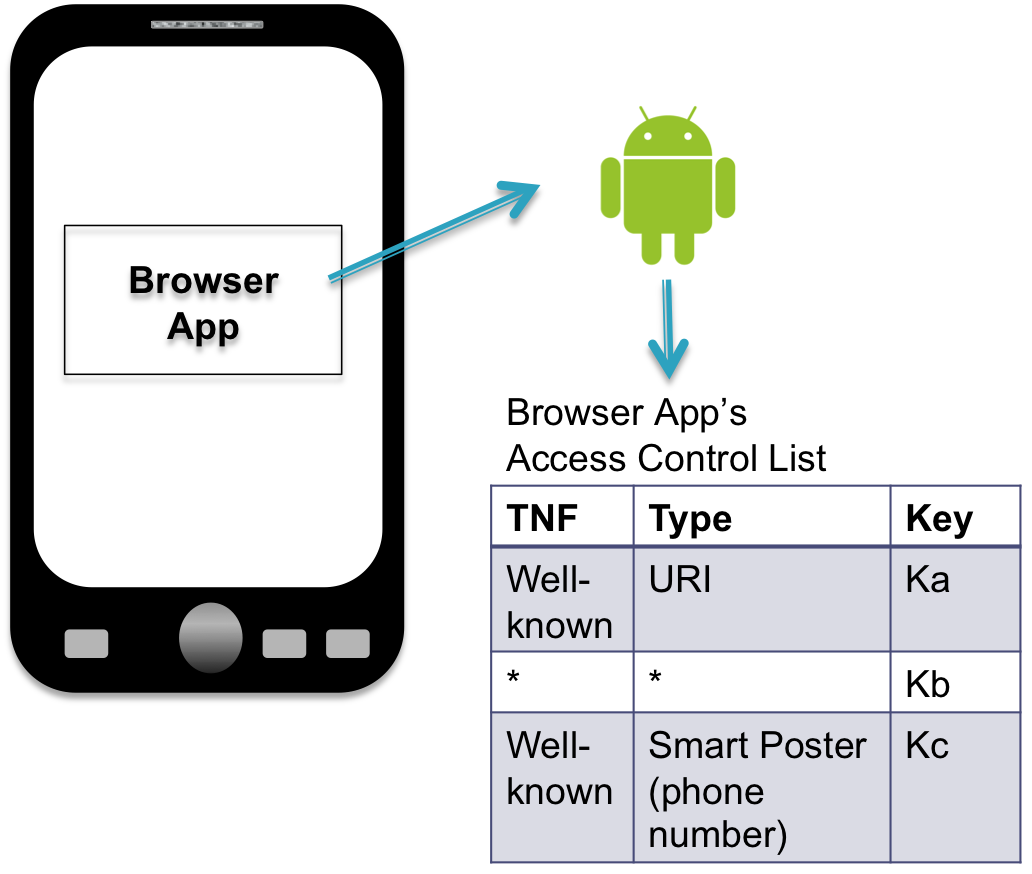
\includegraphics[width=0.5\textwidth]{ACL_image.png}
	\caption[Caption for LOF]%
    {An example of an application's access control list. The Browser application has three entries in its access control list. $K_a$ is a key which is granted access for URI-type tags. $K_b$ is granted access for all tag types. $K_c$ is granted access for phone numbers, found in a Smart Poster tag. The OS manages access verification (including user approval, if necessary) before providing the data to the Browser.}
  \label{fig:solution:acl}

\end{minipage} 
\end{figure}
\subsubsection{Verifying Access}
Before an application can act on NDEF input data, the OS verifies that the NDEF record's type and public key from the associated signature record exist in the access control list.
The format of an entry in the access control list is [TNF:Type:Key].
If such an entry exists, then the key is granted access for the given TNF and Type.
If the OS is able to verify the access of a key and record type, operations will proceed and the NDEF data will be handed to the running application, or launch the relevant application (depending on the current state of the phone).
This content author can either be approved for a specific type (TNF and Type field), or for all types.
For example, an author with public key $K_a$ may have a record [Well-known:URI:$K_a$], indicating that their key is trusted for all URI inputs within the context of that application.
Another author with public key $K_b$ may have a record [*:*:$K_b$], indicating that they will always be granted access by this application.
If the lookup fails, then a user will be prompted to either allow the operation to proceed once (i.e. without granting permanent access), grant permanent access, or deny access and abort the operation.

\subsubsection{Granting Access}
If a user elects to grant access upon receipt of NDEF data, then they will be given the option of granting the tag author permanent access for that NDEF type (TNF and Type fields, or an application-developer-specified type), or for all types (a wildcard match on the TNF and Type fields).
The OS will then attempt to deliver the most readable identifier of the public key which the user is about to approve.
In most cases, extracting the identifying information from the certificate will be sufficient to present the user with a concise identity of the content author.
The user then chooses the type of access they wish to grant to that public key, and this access choice is written to the access control list for that application.

\subsubsection{Revoking Access}
Users will be provided an interface to the access control lists for their applications by the OS.
Through this interface, the user can view all authors to which they have granted access (including the human-readable name associated with the public key).
The user can then choose to revoke access to an author by removing associated entries of that author in relevant lists.
The user can also remove only one access grant to an author, if they so choose.
Revocation should additionally support certificate revocation lists; if a tag with a revoked certificate is encountered, that revocation should propagate to the access control list.
Additionally, if a certificate has been found which is outside its validity period, the access associated with that identity should be revoked by the OS.
Additional information such as most recent access time could be stored in the ACL to aid users in deciding which access rules are no longer necessary.


\subsection{Alternatives}
One access control method we considered was requiring approval when data was handed over to another process, as opposed to approval upon reading the data.
For example, in this scheme if an NFC tag contains a phone number, the user would be prompted to approve the outgoing phone call.
A method such as this could offer persistent approval, as our proposal offers.
After a user approves a phone number to make calls, any further calls would not require further user approval.
We avoid this approach, however, as we feel it is not generalizable in a usable way.
Opening arbitrary URLs presents a significant attack vector in NFC tags.
However, usability of such a scheme decreases drastically if a user must approve every new URL encountered on NFC tags.
The number of tag authors will be lower than the number of resources a user encounters on NFC tags, and as such, author-based access control provides a more generalizable, but still usable, approach.

We considered the merits of allowing access sharing between applications.
The principal benefit of such a system is that there would no longer be duplicate access granting if a user wishes to trust a tag author within the context of multiple applications.
%While this would easily be possible, it raises two major concerns.
%First, shared access control would open the possibility for malicious applications to inject additional trust for authors who may otherwise be untrusted.
%An additional permission for read and write access to the shared access control list would need to be introduced in order to better manage which applications can alter this control list.
There are cases in which sharing access would result in a loss of security.
For example, if one application with limited permissions added a tag author, \textit{A}, as a trusted author for all tag types, this access could be shared with other applications.
If another application with more permissions (such as \texttt{CALL\_PHONE}) saw \textit{A} as having access to all tag types, \textit{A}'s tags would then be able to place phone calls.
There are means to mitigate this threat, but the management becomes significantly more complicated, and simplicity is a necessary facet of our proposal.

We also considered a system in which the OS provided API calls to developers, in which developers would then have to make decisions regarding access.
This system had the potential to grant more flexibility to developers by allowing them to interpret and customize which types were granted access, but the resulting developer overhead would not be worth it.
Our proposal trades minor flexibility for no additional requirements of the developer, and a simple and centralized deployment of access control on the phone.

\section{Implementation}
We began implementing our access control system as an Android library that Android developers can include and access in their projects.
We implemented this as a library only because time constraints would have made it too difficult to implement at OS-level.
Unfortunately, Android does not yet support the NDEF Signature RTD, so much of our work involved working around this.
We provide an API as a proof-of-concept for the proposed access control scheme, through which developers can add, verify, and revoke access.
Our current implementation simply creates a makeshift signature record consisting of a digital signature (created by DSA) and the public key used for the signature.
This emulates the PKI infrastructure provided by certificates, but in a simpler manner, as the focus of our proof-of-concept is the access control itself.
We present this implementation as a proof-of-concept; this proposal must be implemented at OS-level for full effect.
There are several advantages to such OS modifications, which are discussed below.

\subsection{Access Management}
Users need to be able to grant and revoke access to resources, either manually, or in the context of a tag reader application.
For our API, we use Android's \texttt{SharedPreferences}, which provides persistent key-value storage.
Our current implementation provides a unique instance of this access control list (ACL) to an individual application.
%A given application can only access and modify its own access grants (aside from the OS interface provided to the user).
In order to provide an OS library, as well as key management through OS utilities, the access control system must be implemented at OS-level.
The Android Library we implement allows developers to effectively leverage access control, but more features and simplicity would be achieved by integration into Android itself.

\subsection{Recommendations for Kernel Implementation}
We have presented the advantages of an OS implementation of this system.
No additional permissions would be required of this implementation, as applications can only modify their own access control lists.
An application would therefore not be able to falsely influence the access granted on behalf of other applications.
An OS implementation allows for a consolidated and secure means of providing developers with a library for access control, and users with a centralized means of viewing and managing the access they have granted.

\section{Evaluation}
\TODO{Reword/remove.}
In this section we evaluate the feasibility of our suggestions, and their impact on the usability and security of using NFC applications.
Our experience implementing this scheme did not yield any challenges which could not be dealt with.
The largest inhibitor of deployment of this scheme is Android's current lack of support for the NDEF Signature RTD.
While support for this is not strictly necessary for our scheme, which requires only some forms of authentication and integrity, adoption of the Signature RTD standard would be ideal.
Our existing implementation uses a workaround to provide authentication and integrity, which consists of appending a public key and signature to the original NDEF message.
This does not affect the feasibility of our approach, though, as it does not affect the process of administering access control.
We begin building a proof-of-concept application which uses this access control API in order to provide security for reading NFC tags.\footnote{Unfortunately, we had to return the phone we were using for testing, which has currently halted our development.}
This application demonstrates the ease with which access control can be integrated into an NFC application.
As developers do not have to do any additional work, this system is also easier to deploy, and can be deployed on existing phones without adversely affecting application behavior.

\subsection{Similar Systems}
We compare and contrast our proposed design with similar approaches which have been previously implemented.
Each of these systems make some use of certificates or trusted public keys.

\subsubsection{TLS/SSL}
TLS and its predecessor SSL offer authentication via certificate authorities, which allow a user to verify that the web page is being sent by the true owner of the domain.
\subsubsection{Certificates}
Though we do not seek to offer an alternative to the certificate-based authentication used by NDEF signature records, it is worth addressing some issues specific to certificates.
The NDEF Signature RTD supports both X9.68 and X.509 certificates, but both of these are designed for Internet authentication.
NFC tags have limited available space (on the order of kilobytes), but also present a different use case than that of a user connecting to hosts on the Internet.
A user connecting to an Internet host will often have at least some idea of who they are attempting to connect to.
For example, an individual navigating to Google will most likely be able to recognize \url{www.google.com} as the appropriate website.
However, an individual reading an NFC tag may not know the author of that tag before performing the read.
A certificate may associate a name with a public key, but that association may not be useful in the first place\cite{ellison2000}, and may be even less useful to an NFC user.
Certificates can be much more helpful when a user knows who they intend to connect to, and wishes to verify the identity of the individual at the other end of that connection, but NFC tags dictate who is providing the content.

\subsubsection{Java Applets and ActiveX}
A signed Java applet includes a digital signature of the Java binary that can be verified with a certificate belonging to the applet author.
Signed Java applets have more capabilities than unsigned applets and run outside of the sandbox and essentially have full access to the user's computer.
When a user navigates to a web page containing a signed Java applet, the user is prompted with a warning asking if the user trusts the certificate, either temporarily or permanently.
If the user chooses to accept the certificate permanently, then \textit{any} applet signed with the same key can be run automatically with full permissions.
This represents an ``all-or-nothing'' mentality in which an author is either completely denied access or granted full access.
In contrast, we offer the user the ability to grant a tag author access to a \textit{particular} resource.
ActiveX offers essentially the same mechanism as Java applets.

\subsubsection{SSH}
The Secure Shell (SSH) protocol asks users to authenticate the host to which they are connecting by examining a digest of the host's public key.
After accepting this key, the host and corresponding key are stored, so that a user need not authenticate the host's public key again.
This differs from the previous two examples in that there is less certification overhead at the expense of a greater burden on the user to trust the right host.
In addition, the user does not grant the server authorization to any local resources, which results in a different threat model than that of NFC.
We offer users the ability to trust an author once and avoid future prompts for authorization, but our system offers more power to the user by providing them with information regarding the author (and not just a digest of the author's public key).

\subsection{Use Case: Smart Poster}
Smart posters\footnote{\url{http://www.nfc-forum.org/resources/presentations/NFC_Smart_Poster_WIMA_2011.pdf}} are a common application of NFC tags where a normal poster is augmented with an NFC tag that provides additional data.
For this example we consider movie poster campaign which provides more information to potential moviegoers, such as similar campaign in 2011\footnote{\url{http://www.nfcworld.com/2011/05/23/37591/x-men-nfc-smart-poster-london/}}.
A malicious user could remove or disable the existing tag and replace it with his or her own tag, which could automatically place a phone call to a tolled number.
Under the existing scheme, a user's phone would automatically place the phone call without prompting the user, causing the user to spend money.
Under our scheme, a user would see that the tag is not signed by a key that they trust, and they would have to add the key.
If the user had already added a key belonging to the organization that created the poster, they would become suspicious of the fact that there is a new key associated with the current poster.
As there is probably a centralized producer of smart posters in many cases, and specifically in this example, once a poster is trusted, a user can scan any other smart poster made by the same company without worrying again. 
Additionally, as we allow finer-grained access to these tags, if the advertising company's perogative was to instead call a tolled phone number that they provide on the signed tag, our system would prevent the malicious tag writer's attack. The user would have only allowed the movie poster access to certain permissions, not including the CALL PHONE permission in this case.  

\subsection{Usability}
NFC offers a unique means of quickly performing actions via a single swipe of a tag; to this end, any security solution must therefore be particularly mindful of the tradeoffs between usability and security.
Our recommendations focus on minimizing the additional interaction required of a user to add more security to their NFC transactions.
Users should be offered the option to approve a tag's author permanently (by updating the access control list), as well as to grant the author access on a case-by-case basis.
Additionally, to ensure backwards compatibility, unsigned NFC tags should not cause the system to break.
We recommend giving users a choice regarding the handling of an unsigned tag.
The most secure means of supporting tags without signature records is to warn the user and prompt for approval every time such a tag is encountered.
However, this severely inhibits the ease of use of an NFC application.
Additionally, this behavior would likely result in users being trained to ignore warnings.
We have not yet found an optimal solution for dealing with unsigned tags, although a balance between usability and security would be to only prompt the user for access approval if the tag types are of high security value, such as a phone number or URL.
%This could be subverted, though, and would likely result in high false positives and high false negatives in warnings.
One option would be to have a per-application or per-tag-type policy for handling unsigned tags, since a user may want greater security for certain applications and not others.
In Section~\ref{sec:futurework} we consider how to test the usability of access control in the presence of both signed and unsigned applications.

\subsection{Security}
The operating system takes care of the access control, so there is no need for additional development of applications, and no risk of developers improperly using (or simply not using) a framework.
As the NFC application landscape for Android is still growing, it remains to be seen how many applications will benefit from this additional security.

\section{Future Work}
\label{sec:futurework}
The next major step for this scheme is its implementation at operating system level.
An OS implementation is required to keep access control decisions from complicating application logic, as well to provide access control administration interface to the user.
This implementation will make for a more detailed evaluation, as there will be no more speculation about the functionality of the system.
It will also not be difficult to address some of the issues we presented in Section~\ref{sec:threatmodel:privacy}.
At the very least, when a user writes a tag which they wish to be used by their phone only, they should be provided the option to encrypt and verify the integrity of that tag.
The Android NDEF API could offer this encryption to developers of tag-writing applications, who could then offer the feature to the user.
Encryption would prevent leaks of private information from NFC tags even if the physical tag were to be compromised.
%We would also like to explore further generalization of this access control system, and its potential in areas other than NFC inputs.


\subsection{Recommended User Study}
NFC is still emerging in smart phones, and as such there are uses and applications of NFC which have yet to be seen.
However, there are still several common use cases which are already deployed or in the process of being adopted.
In the future, we would like to examine common and expected use cases of NFC, and how access controls can provide improved security for these cases.
We present some features of a user study which would evaluate the obtrusiveness and effectiveness of access controls in a realistic setting.

The goal of such a user study is to provide a quantitative evaluation of the usability overhead imposed by warning and approval messages which result from employing our access control system, as well as the effectiveness of this system in mitigating attacks.
We would like to test a breadth of NFC applications which exhibit a range of complexity and potential for attack.
Applications which we think would be interesting for this include a SmartPoster application, an application for purchasing a bus ticket (using SMS for payment), and an application which allows NFC-grocery-shopping.
We would further like to evaluate these applications, and our system, in the presence of unsigned tags and signed tags, with malicious tags present in both cases.
We are still evaluating the most accurate way to measure the usability and security effectiveness of our system's deployment.
NFC demands certain levels of usability, and through a user study we seek to ensure that our system provides such levels while still offering acceptable security.
Further evaluation of the tradeoffs of usability and security in the context of NFC applications will be crucial to the adoption of our system (or any system which seeks to provide usable security for NFC applications).


{\section{Conclusion}
NFC applications and NFC-enabled devices are becoming increasingly popular, and with this popularity will come the attention of attackers.
We have examined the NFC Data Exchange Format, and in particular its deployment in Android.
We consider the NDEF Signature RTD, and its uses for providing integrity and authentication.
From this authentication, we propose a system to provide authorization, via access control lists dictating the access granted to tag authors for specific tag types.
We partially implement this system, and evaluate its usability and security.
This access control system addresses several issues present in NFC applications which cannot be directly addressed by signature records alone.

\section{Acknowledgements}
We would like to thank Dawn Song and her research group for letting us borrow an NFC-enabled Android phone.


\bibliographystyle{acm}
\bibliography{cs261}

\end{document}
